\documentclass[manual-fr.tex]{subfiles}
\begin{document}

To make process simpler, SEM disallows the user to modify the content of the files or modify a loaded tagset. To annotate a document, the following should be done:
\begin{itemize}
    \item load the document from a file;
    \item load the tagset from a file;
\end{itemize}

~

SEM will generate keyboard shortcuts from the loaded tagset. A tagset is a text file containing one tag per line, such as the following:

\begin{lstlisting}[frame=single]
tag1

# a comment
tag2.subtag1
tag2.subtag2 # another comment

tag3
\end{lstlisting}

SEM handles hierarchical tags and considers the caracter '.' as the separator between levels. Empty lines are ignored and the character "\#" allows to write comment that will be ignored. In our case, we wish to handle the tags \emph{software} ("logiciel" in the figures) and \emph{person} ("personne" in the figures). The tagset file will then have the following content :

\begin{lstlisting}[frame=single]
software
person
\end{lstlisting}

Figures \ref{fig:annotation_sem-02} and \ref{fig:annotation_sem-03} show how to load a document and a tagset.

\begin{figure}[ht!]
    \begin{center}
    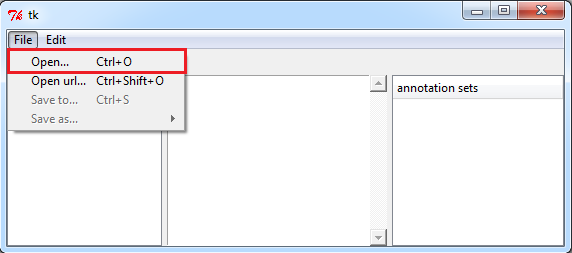
\includegraphics[scale=0.5]{fr/images/annotation_sem-02.png}
    \end{center}
    \caption{Framed in red : the menu element to load a document.}
    \label{fig:annotation_sem-02}
\end{figure}



\begin{figure}[ht!]
    \begin{center}
    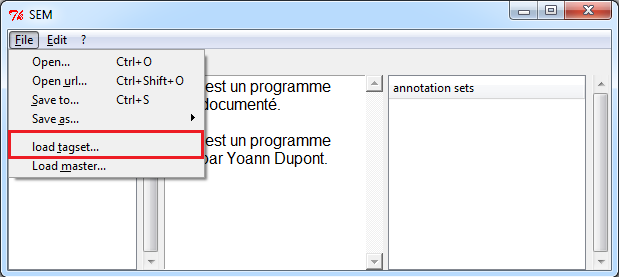
\includegraphics[scale=0.5]{fr/images/annotation_sem-03.png}
    \end{center}
    \caption{Framed in red : the button to load a tagset.}
    \label{fig:annotation_sem-03}
\end{figure}


Figures \ref{fig:annotation_sem-04}, \ref{fig:annotation_sem-05} and \ref{fig:annotation_sem-06} how to manually annotate a corpus then retrain a model SEM can use with this corpus.


\begin{figure}[ht!]
    \begin{center}
    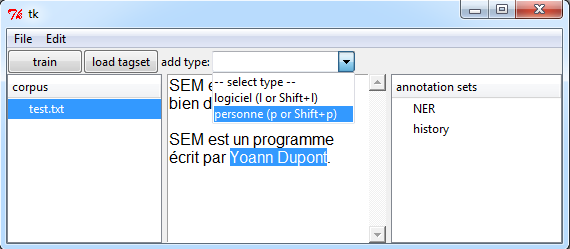
\includegraphics[scale=0.5]{fr/images/annotation_sem-04.png}
    \end{center}
    \caption{To annotate an element: select the text and choose the tag in the list (which gives the keyboard shortcuts).}
    \label{fig:annotation_sem-04}
\end{figure}



\begin{figure}[ht!]
    \begin{center}
    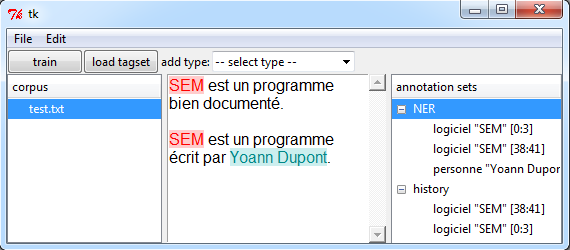
\includegraphics[scale=0.5]{fr/images/annotation_sem-05.png}
    \end{center}
    \caption{To annotate all occurrences in the document : use keyboard shortcut $<Shift+\_>$ where "\_" is the keyboard shortcut for the tag. If we look at figure \ref{fig:annotation_sem-04}, $<Shift+l>$ allows to annotate all occurrences of "SEM" as "software".}
    \label{fig:annotation_sem-05}
\end{figure}



\begin{figure}[ht!]
    \begin{center}
    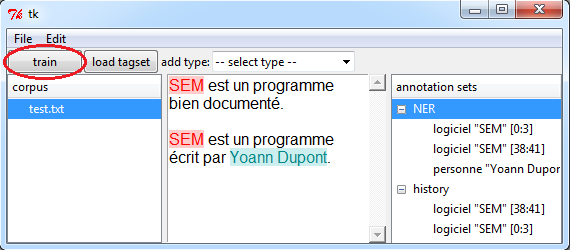
\includegraphics[scale=0.5]{fr/images/annotation_sem-06.png}
    \end{center}
    \caption{Framed in red : the button to train SEM with the corpus and its current annotations. The interface is identical to the one shown in section \ref{subsubsec:train-SEM-from-annotated}.}
    \label{fig:annotation_sem-06}
\end{figure}

\end{document}
